\section{Systemaufbau}
Der Laboraufbau besteht aus einer Siemens S7-1500 Steuerung und mehreren Peripheriegeräten, die teils direkt, teils über Feldbus-Master angebunden sind. 
Tabelle~\ref{tab:hw} gibt einen Überblick über die verwendeten Hardwarekomponenten, Abbildung~\ref{fig:topologie} zeigt ihre Vernetzung in der Topologieansicht des TIA Portals und Abbildung~\ref{fig:anzeigeeinheit} den realen Laboraufbau mit der Anzeigeeinheit.

\begin{table}[H]
\centering\small
\begin{tabular}{|L{3.0cm}|L{3.8cm}|L{7.2cm}|}
\hline
\textbf{Komponente} & \textbf{Typ} & \textbf{Funktion} \\ \hline
SPS & S7-1500 (CPU 1512) & Zentrale Steuerung des Anwenderprogramms \\ \hline
Ethernet-Switch & Scalance XB005 & Verbindet CPU und Feldbus-Master über PROFINET \\ \hline
IO-Link-Master & ifm AL1100 & Bindet IO-Link-Geräte an PROFINET an \\ \hline
AS-i-Master & ifm AC1401 & Bindet AS-i-Slaves an PROFINET an \\ \hline
Optischer Sensor & ifm O8T202 & Erkennt den Zeiger in der Referenzposition (IO-Link) \\ \hline
Leuchttaster & ifm AC2398 & Zwei Taster (grün, rot) mit LEDs zur Bedienung (AS-i) \\ \hline
Temperatursensor & PT100 + Messumformer & Temperaturmessung, 0--10\,V-Signal am Analogeingang \\ \hline
Schrittmotor & Schrittmotor + Treiber & Bewegt den Anzeigepfeil, Ansteuerung über Takt und Drehrichtung \\ \hline
\end{tabular}
\caption{Verwendete Hardwarekomponenten}
\label{tab:hw}
\end{table}

Die Anbindung an die SPS erfolgt auf drei Wegen. 
Der Leuchttaster AC2398 mit seinen Tastern und Leuchtmitteln wird über den AS-i-Master AC1401 in das System eingebunden, der die AS-i-Daten über PROFINET an die SPS weitergibt. 
Der optische Sensor O8T202 ist an den IO-Link-Master AL1100 angeschlossen, der ebenfalls über PROFINET mit der SPS kommuniziert. 
Der Schrittmotortreiber und damit der Motor sind dagegen direkt über zwei Digitalausgänge (DQ) der Steuerung verdrahtet, ebenso ist der PT100 über seinen Messumformer direkt am Analogeingang angeschlossen.

% Topologieansicht aus dem TIA Portal als images/Topologie.png ablegen
\begin{figure}[H]
    \centering
    \IfFileExists{images/TopologieansichtTIA.png}{%
        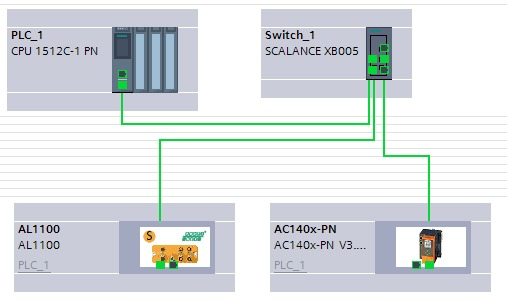
\includegraphics[width=\textwidth, height=0.3\textheight, keepaspectratio]{images/TopologieansichtTIA.png}%
    }{\fbox{\parbox[c][6cm][c]{0.9\textwidth}{\centering Topologieansicht TIA Portal folgt}}}
    \caption{Topologieansicht des Projekts im TIA Portal}
    \label{fig:topologie}
\end{figure}

% Foto des Laboraufbaus mit Schrittmotor, Skala und Anzeigepfeil
\begin{figure}[H]
    \centering
    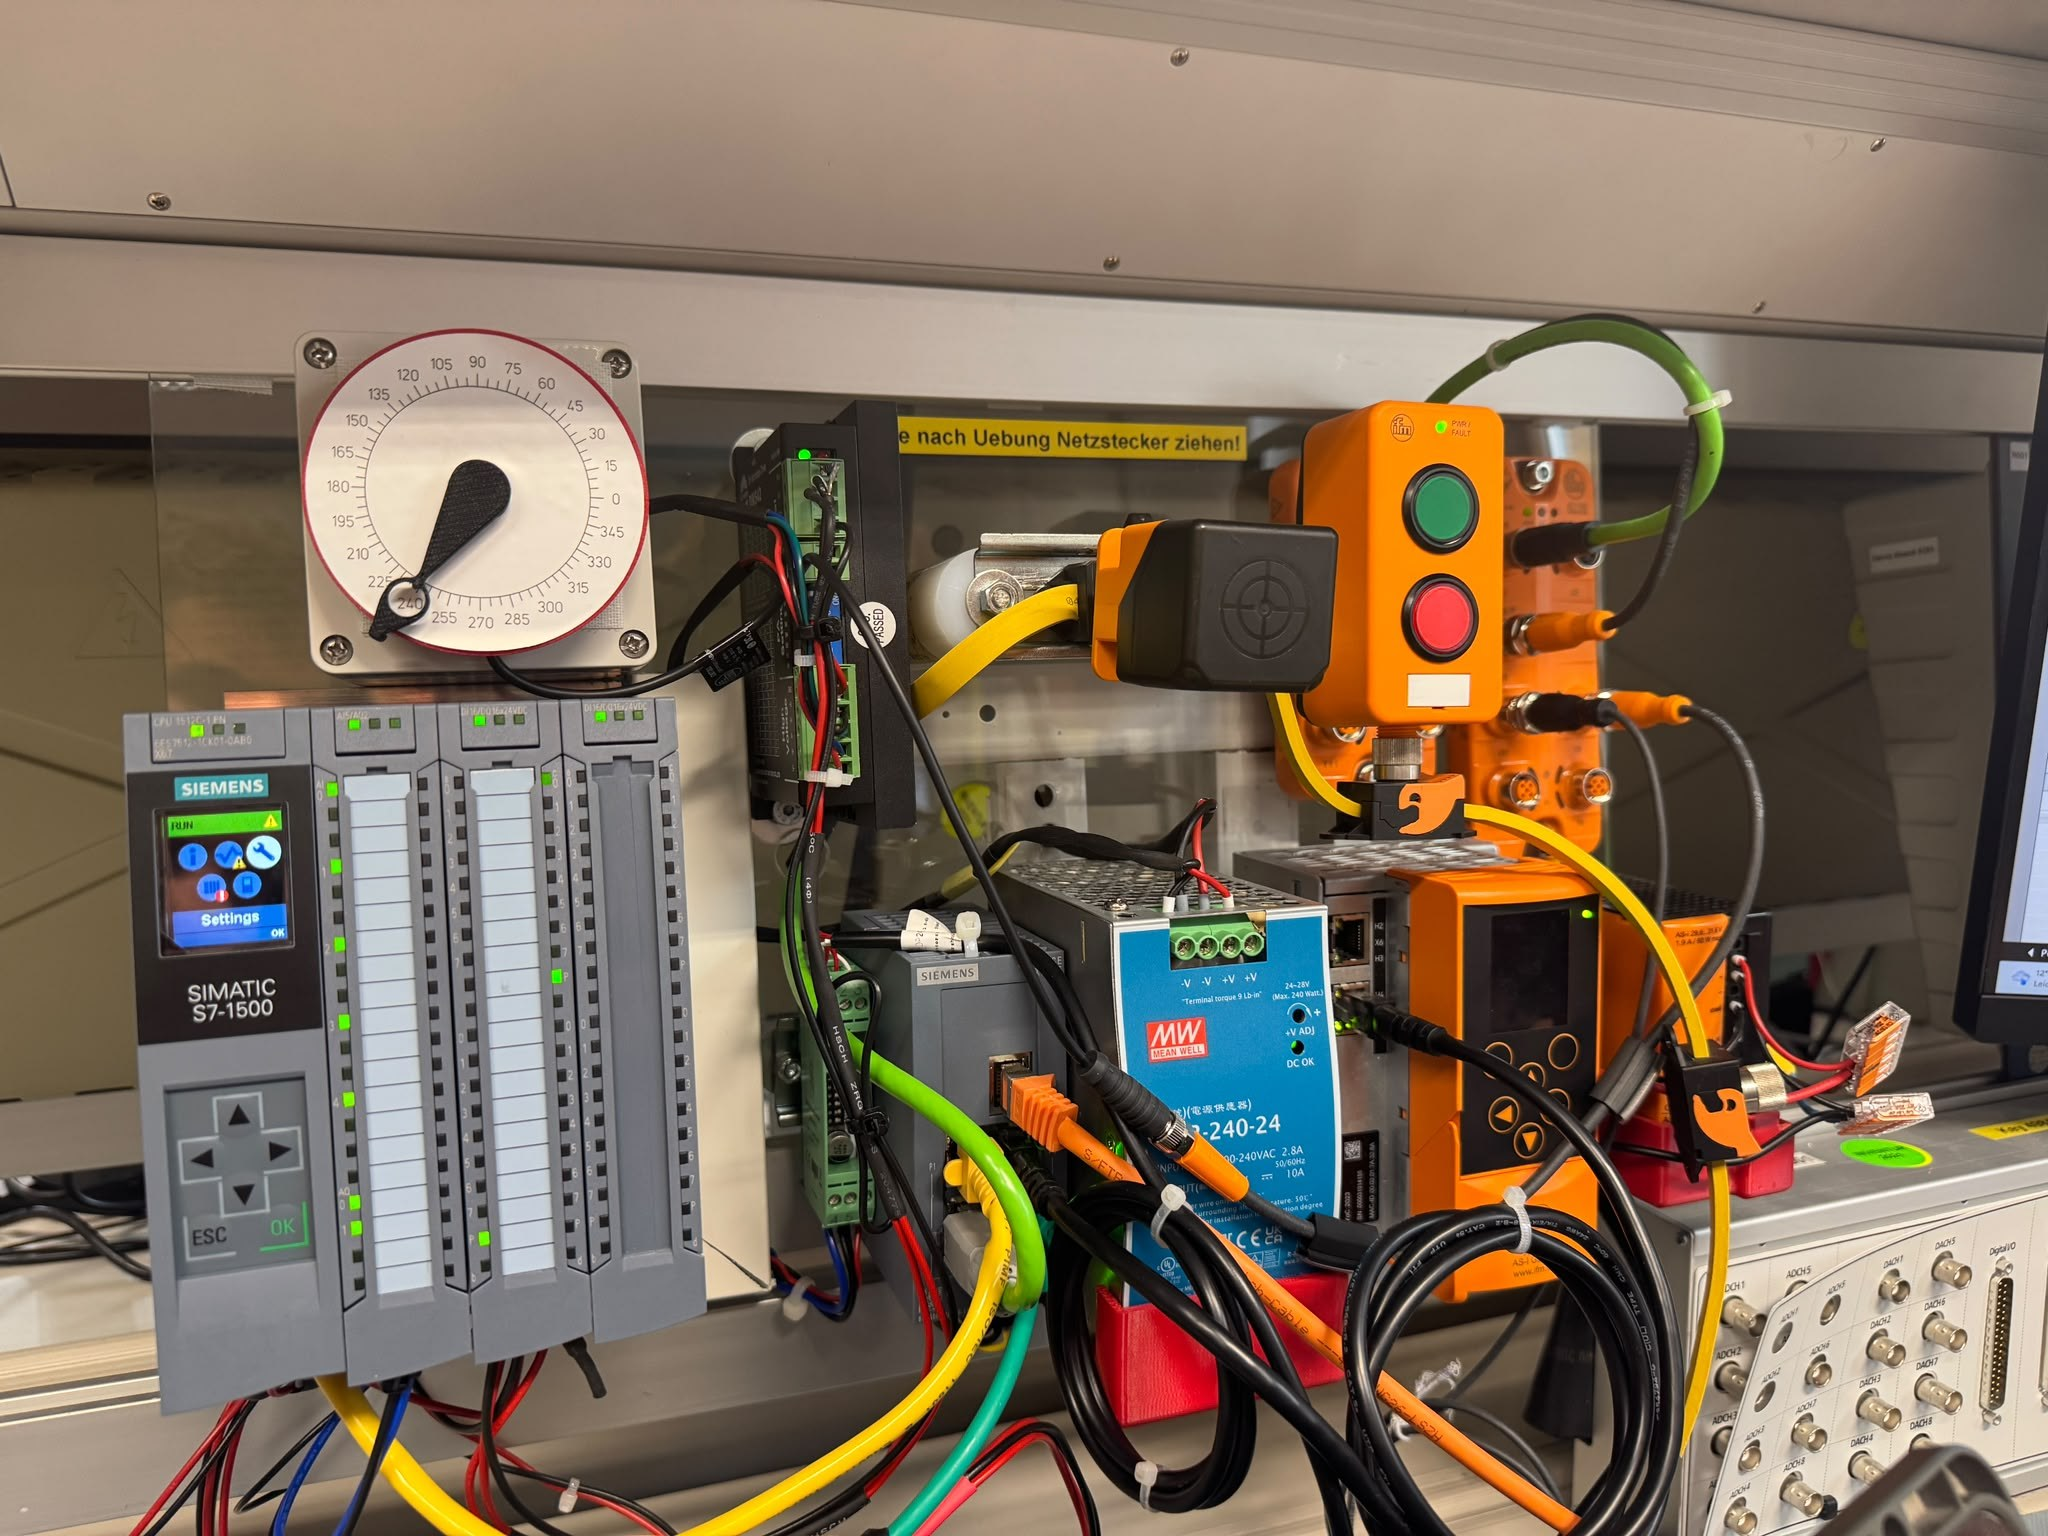
\includegraphics[width=0.85\textwidth]{images/Laboraufbau.jpg}
    \caption{Laboraufbau mit Schrittmotor, montierter Skala und Anzeigepfeil (oben links)}
    \label{fig:anzeigeeinheit}
\end{figure}
